\PassOptionsToPackage{unicode=true}{hyperref} % options for packages loaded elsewhere
\PassOptionsToPackage{hyphens}{url}
%
\documentclass[]{article}
\usepackage{lmodern}
\usepackage{amssymb,amsmath}
\usepackage{ifxetex,ifluatex}
\usepackage{fixltx2e} % provides \textsubscript
\ifnum 0\ifxetex 1\fi\ifluatex 1\fi=0 % if pdftex
  \usepackage[T1]{fontenc}
  \usepackage[utf8]{inputenc}
  \usepackage{textcomp} % provides euro and other symbols
\else % if luatex or xelatex
  \usepackage{unicode-math}
  \defaultfontfeatures{Ligatures=TeX,Scale=MatchLowercase}
\fi
% use upquote if available, for straight quotes in verbatim environments
\IfFileExists{upquote.sty}{\usepackage{upquote}}{}
% use microtype if available
\IfFileExists{microtype.sty}{%
\usepackage[]{microtype}
\UseMicrotypeSet[protrusion]{basicmath} % disable protrusion for tt fonts
}{}
\IfFileExists{parskip.sty}{%
\usepackage{parskip}
}{% else
\setlength{\parindent}{0pt}
\setlength{\parskip}{6pt plus 2pt minus 1pt}
}
\usepackage{hyperref}
\hypersetup{
            pdftitle={Experiments in Generative Evolution},
            pdfauthor={Simon Hickinbotham},
            pdfborder={0 0 0},
            breaklinks=true}
\urlstyle{same}  % don't use monospace font for urls
\usepackage[margin=1in]{geometry}
\usepackage{color}
\usepackage{fancyvrb}
\newcommand{\VerbBar}{|}
\newcommand{\VERB}{\Verb[commandchars=\\\{\}]}
\DefineVerbatimEnvironment{Highlighting}{Verbatim}{commandchars=\\\{\}}
% Add ',fontsize=\small' for more characters per line
\usepackage{framed}
\definecolor{shadecolor}{RGB}{248,248,248}
\newenvironment{Shaded}{\begin{snugshade}}{\end{snugshade}}
\newcommand{\AlertTok}[1]{\textcolor[rgb]{0.94,0.16,0.16}{#1}}
\newcommand{\AnnotationTok}[1]{\textcolor[rgb]{0.56,0.35,0.01}{\textbf{\textit{#1}}}}
\newcommand{\AttributeTok}[1]{\textcolor[rgb]{0.77,0.63,0.00}{#1}}
\newcommand{\BaseNTok}[1]{\textcolor[rgb]{0.00,0.00,0.81}{#1}}
\newcommand{\BuiltInTok}[1]{#1}
\newcommand{\CharTok}[1]{\textcolor[rgb]{0.31,0.60,0.02}{#1}}
\newcommand{\CommentTok}[1]{\textcolor[rgb]{0.56,0.35,0.01}{\textit{#1}}}
\newcommand{\CommentVarTok}[1]{\textcolor[rgb]{0.56,0.35,0.01}{\textbf{\textit{#1}}}}
\newcommand{\ConstantTok}[1]{\textcolor[rgb]{0.00,0.00,0.00}{#1}}
\newcommand{\ControlFlowTok}[1]{\textcolor[rgb]{0.13,0.29,0.53}{\textbf{#1}}}
\newcommand{\DataTypeTok}[1]{\textcolor[rgb]{0.13,0.29,0.53}{#1}}
\newcommand{\DecValTok}[1]{\textcolor[rgb]{0.00,0.00,0.81}{#1}}
\newcommand{\DocumentationTok}[1]{\textcolor[rgb]{0.56,0.35,0.01}{\textbf{\textit{#1}}}}
\newcommand{\ErrorTok}[1]{\textcolor[rgb]{0.64,0.00,0.00}{\textbf{#1}}}
\newcommand{\ExtensionTok}[1]{#1}
\newcommand{\FloatTok}[1]{\textcolor[rgb]{0.00,0.00,0.81}{#1}}
\newcommand{\FunctionTok}[1]{\textcolor[rgb]{0.00,0.00,0.00}{#1}}
\newcommand{\ImportTok}[1]{#1}
\newcommand{\InformationTok}[1]{\textcolor[rgb]{0.56,0.35,0.01}{\textbf{\textit{#1}}}}
\newcommand{\KeywordTok}[1]{\textcolor[rgb]{0.13,0.29,0.53}{\textbf{#1}}}
\newcommand{\NormalTok}[1]{#1}
\newcommand{\OperatorTok}[1]{\textcolor[rgb]{0.81,0.36,0.00}{\textbf{#1}}}
\newcommand{\OtherTok}[1]{\textcolor[rgb]{0.56,0.35,0.01}{#1}}
\newcommand{\PreprocessorTok}[1]{\textcolor[rgb]{0.56,0.35,0.01}{\textit{#1}}}
\newcommand{\RegionMarkerTok}[1]{#1}
\newcommand{\SpecialCharTok}[1]{\textcolor[rgb]{0.00,0.00,0.00}{#1}}
\newcommand{\SpecialStringTok}[1]{\textcolor[rgb]{0.31,0.60,0.02}{#1}}
\newcommand{\StringTok}[1]{\textcolor[rgb]{0.31,0.60,0.02}{#1}}
\newcommand{\VariableTok}[1]{\textcolor[rgb]{0.00,0.00,0.00}{#1}}
\newcommand{\VerbatimStringTok}[1]{\textcolor[rgb]{0.31,0.60,0.02}{#1}}
\newcommand{\WarningTok}[1]{\textcolor[rgb]{0.56,0.35,0.01}{\textbf{\textit{#1}}}}
\usepackage{graphicx,grffile}
\makeatletter
\def\maxwidth{\ifdim\Gin@nat@width>\linewidth\linewidth\else\Gin@nat@width\fi}
\def\maxheight{\ifdim\Gin@nat@height>\textheight\textheight\else\Gin@nat@height\fi}
\makeatother
% Scale images if necessary, so that they will not overflow the page
% margins by default, and it is still possible to overwrite the defaults
% using explicit options in \includegraphics[width, height, ...]{}
\setkeys{Gin}{width=\maxwidth,height=\maxheight,keepaspectratio}
\setlength{\emergencystretch}{3em}  % prevent overfull lines
\providecommand{\tightlist}{%
  \setlength{\itemsep}{0pt}\setlength{\parskip}{0pt}}
\setcounter{secnumdepth}{0}
% Redefines (sub)paragraphs to behave more like sections
\ifx\paragraph\undefined\else
\let\oldparagraph\paragraph
\renewcommand{\paragraph}[1]{\oldparagraph{#1}\mbox{}}
\fi
\ifx\subparagraph\undefined\else
\let\oldsubparagraph\subparagraph
\renewcommand{\subparagraph}[1]{\oldsubparagraph{#1}\mbox{}}
\fi

% set default figure placement to htbp
\makeatletter
\def\fps@figure{htbp}
\makeatother


\title{Experiments in Generative Evolution}
\author{Simon Hickinbotham}
\date{12/01/2021}

\begin{document}
\maketitle

\hypertarget{terminologystrategy}{%
\subsection{Terminology/strategy}\label{terminologystrategy}}

\begin{itemize}
\tightlist
\item
  grow a network of ``undifferentiated cells'' as ``undifferentiated
  nodes'' (u-nodes) connected by ``undifferenitated edges'' (u-edges)
\item
  each iteration, check for proximity to a stimulus
\item
  once a stimulus is found, propagate the info back to the foundation
\item
  reinforce edges that make this link
\item
  reposition edges that make this link to support them
\end{itemize}

\hypertarget{setting-up}{%
\subsection{Setting up}\label{setting-up}}

Ideally we'd try to grow from a single foundation, and have a ``stimulus
point'' that triggers conversion from sensing nodes to support nodes.
But since determining where to grow - even randomly - is complicated,
we'll start with a uniform grid of cells. This is potentially wasteful
but it allows us to get to solving the main issues early.

\hypertarget{node-types}{%
\subsection{Node types}\label{node-types}}

\begin{itemize}
\tightlist
\item
  ``U'': undifferentiated - all nodes start like this
\item
  ``F'': foundation - build from here - these are set manually after
  initialising
\item
  ``S'': a node near to or linked to a stimulus - which can be a set
  point or another network
\item
  ``X'': an undifferentiated node that is located in an inhibition
  region
\item
  ``C'': a constructor node - basis of converting to solid structure
\end{itemize}

\hypertarget{regular-network-version}{%
\subsection{Regular network version}\label{regular-network-version}}

Adding nodes on a grid is pretty straghtforward. Here we'll create a
regular square lattice with cross-braces. We commence with the nodes:

\begin{Shaded}
\begin{Highlighting}[]
\KeywordTok{source}\NormalTok{(}\StringTok{"maycode.R"}\NormalTok{)}
\end{Highlighting}
\end{Shaded}

Now the edges. Let's start by using integers only, cos then we can
predict the position and we don't have to minimise any distances to find
neighbours. Here's a function \texttt{addedge} to add an edge to the
set:

Now we can generate a regular network within and x,y range - the process
will be similar for 3D - we'd just have to add a z dimension.

\begin{Shaded}
\begin{Highlighting}[]
\CommentTok{# constants}
\NormalTok{iel =}\StringTok{ }\DecValTok{50}            \CommentTok{# ideal edge length - not used yet}
\NormalTok{xlim =}\StringTok{ }\KeywordTok{c}\NormalTok{(}\OperatorTok{-}\DecValTok{100}\NormalTok{,}\DecValTok{100}\NormalTok{)  }\CommentTok{# x range}
\NormalTok{ylim =}\StringTok{ }\KeywordTok{c}\NormalTok{(}\DecValTok{0}\NormalTok{,}\DecValTok{200}\NormalTok{)     }\CommentTok{# y range}
\NormalTok{ostep =}\StringTok{ }\DecValTok{20}

\NormalTok{net <-}\StringTok{ }\KeywordTok{makenet}\NormalTok{(xlim,ylim,ostep)}

\CommentTok{# Set the foundation nodes: }
\CommentTok{#net$n$type[net$n$n>=5 & net$n$n <=7]<-"F"}
\NormalTok{net <-}\StringTok{ }\KeywordTok{setnodetype}\NormalTok{(net,}\OperatorTok{-}\DecValTok{25}\NormalTok{,}\OperatorTok{-}\DecValTok{5}\NormalTok{,}\DecValTok{25}\NormalTok{,}\DecValTok{5}\NormalTok{,}\StringTok{"F"}\NormalTok{)}
 
\CommentTok{# Store the network's initial state:}
\NormalTok{innet <-}\StringTok{ }\NormalTok{net}

\CommentTok{# Here's a stimulus: }
\NormalTok{stim <-}\StringTok{ }\KeywordTok{data.frame}\NormalTok{(}\DataTypeTok{x=}\OperatorTok{-}\DecValTok{5}\NormalTok{,}\DataTypeTok{y=}\DecValTok{145}\NormalTok{)}
\end{Highlighting}
\end{Shaded}

If we eventually want an irregular network then an alternative to the
above would be to generate a set of random nodes in the space and then
connect the edges via e.g.~a Delaunay triangulation. Hard to say what
the advantage of this would be right now, but later on it may be a
better way to initialise so we can get the system robust to stochastic
effects.

\hypertarget{growing-the-network-levels}{%
\subsection{Growing the network
levels}\label{growing-the-network-levels}}

Here's the initial network: a foundation of two connected nodes

Let's have a function to plot the network - we'll use this to keep track
of how the network grows later. The bottom of this code block shows the
initial network:

\begin{Shaded}
\begin{Highlighting}[]
\KeywordTok{plotnet}\NormalTok{(net,stim,}\DataTypeTok{xlim=}\NormalTok{xlim,}\DataTypeTok{ylim=}\NormalTok{ylim)}
\end{Highlighting}
\end{Shaded}

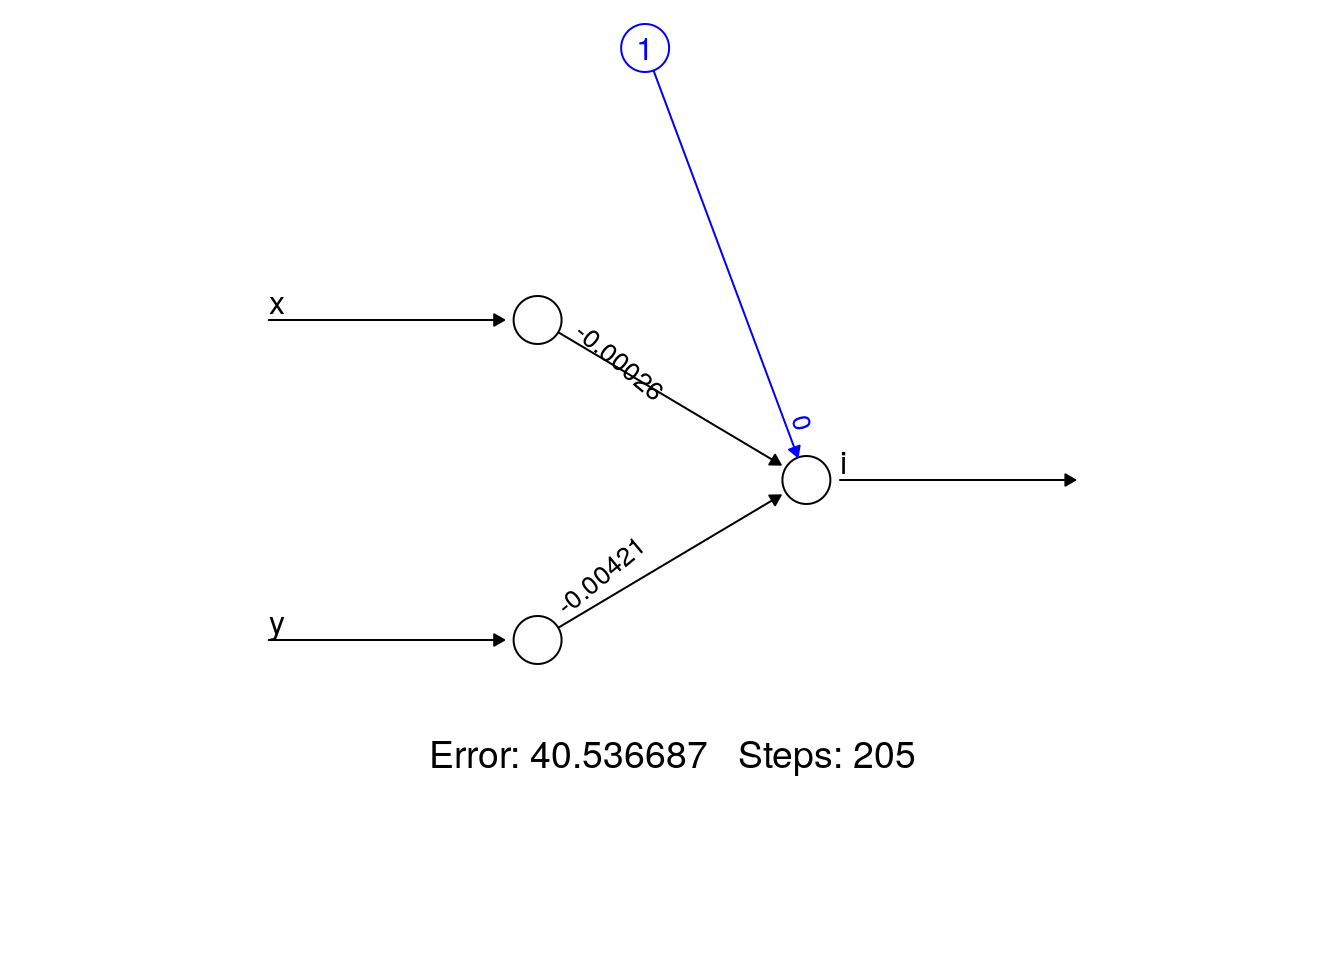
\includegraphics{mayprojtest_files/figure-latex/unnamed-chunk-3-1.pdf}

Here's the \texttt{propagate} function to grow the network:

Here are functions to check whether a stimulus has been reached by a net
(\texttt{checkstim}), and to propagate that information back to the
foundation (\texttt{propstim}):

OK that's a good start - we need to propagate the connectivity between
the foundation and the stimulus

\begin{Shaded}
\begin{Highlighting}[]
\CommentTok{#for (i in 1:10) \{}
\CommentTok{#    plot(x=i/2, y=i/2, xlim=c(0,6), ylim=c(0,6), pch=20, col=palette()[2], cex=5)}
\CommentTok{#\}}




\NormalTok{nl <-}\StringTok{ }\KeywordTok{list}\NormalTok{()}
\NormalTok{nl[[}\DecValTok{1}\NormalTok{]]<-innet}

\NormalTok{nl =}\StringTok{ }\KeywordTok{rungrowth}\NormalTok{(nl, }\DataTypeTok{stim =}\NormalTok{ stim,}\DataTypeTok{inhib=}\OtherTok{NULL}\NormalTok{, }\DataTypeTok{nsteps =} \DecValTok{15}\NormalTok{,}\DataTypeTok{xlim=}\NormalTok{xlim,}\DataTypeTok{ylim=}\NormalTok{ylim)}
\end{Highlighting}
\end{Shaded}

\animategraphics[,controls,loop]{5}{mayprojtest_files/figure-latex/linkit2-}{1}{15}

\begin{Shaded}
\begin{Highlighting}[]
\CommentTok{#net = rungrowth(net = innet, stim = stim, nsteps = 15, xlim=xlim,ylim=ylim)}
\end{Highlighting}
\end{Shaded}

\hypertarget{other-stimulus-examples}{%
\subsection{Other stimulus examples:}\label{other-stimulus-examples}}

let's do a stimulus in various different positions. Because the lattice
is not symmetrical, there'll be some positional effects - again, let's
worry about those later when we've got the main network growing. Here's
a stimulus to the left of the foundation, which has to run perpendicular
to the edge diagonals

\animategraphics[,controls,loop]{5}{mayprojtest_files/figure-latex/linkit3-}{1}{20}

\ldots{}and here's one to the right, which has to run parallel to the
diagonals. You can see there's a different effect on how the network
grows.

\animategraphics[,controls,loop]{5}{mayprojtest_files/figure-latex/linkit-}{1}{15}

\hypertarget{obstacles}{%
\section{Obstacles}\label{obstacles}}

OK, now to start to hit the bridge challenge, we need to specify the
void under the bridge. We'll do this via a list of rectangles - this
will make it easier to code for in this proof-of-concept stage. I've
updated the \texttt{plotnet} function to draw obstacles in dark grey
behind the network. The next code chunk creates a wider network with a
void region, and plots it:

\animategraphics[,controls,loop]{5}{mayprojtest_files/figure-latex/obst1-}{1}{36}

\animategraphics[,controls,loop]{5}{mayprojtest_files/figure-latex/obst2-}{1}{41}

\hypertarget{multiple-networks-and-stimuli}{%
\section{Multiple networks and
stimuli}\label{multiple-networks-and-stimuli}}

A key concept is that a node from another network should work exactly
like a stimulus. The issue then is how to keep track of stimlevels etc.

Let's refactor everything so we have a bunch of different networks and
see how they meet each other around obstacles. Then we can understand
what's going on.

\animategraphics[,controls,loop]{5}{mayprojtest_files/figure-latex/unnamed-chunk-7-}{1}{43}

OK, this \emph{kind of} works, but the code is getting unwieldy and
there's a lot of redundancy in the way the networks overlap. I can also
forsee problems in joining the networks together if we go down this
route.

I think a better approach is to have a \emph{single} network of nodes,
but to allow for more than one instance of a node type. So each node has
a type (say ``F''), and a type index - so we can have more than one
Foundation node cluster - in the above image we'd have tidx of 1 for the
left side and 2 for the right side. As the levels grow out, we'd keep
track of which ``F'' the level pertains to. What remains to be
discovered is how

\hypertarget{how-does-evolution-fit-into-this}{%
\section{How does evolution fit into
this}\label{how-does-evolution-fit-into-this}}

I think we are heading for the situation where each node is governed by
a kind of gene-regulatory network, whereby each node updates its state
based on information coming from the edges that connect to it and the
switching on and off of genes to generate responses.

\begin{center}\rule{0.5\linewidth}{0.5pt}\end{center}

\hypertarget{obsolete-code}{%
\section{Obsolete code}\label{obsolete-code}}

Here are some functions I tried but that didn't go anywhere (yet)

\hypertarget{growing-the-network-from-scratch}{%
\paragraph{Growing the network from
scratch}\label{growing-the-network-from-scratch}}

I did a little work on actually growing the network, rather than
establishing a grid that covers the whole space.

Here's the initial network: a foundation of two connected nodes

\begin{Shaded}
\begin{Highlighting}[]
\CommentTok{# constants}
\NormalTok{iel =}\StringTok{ }\DecValTok{50}

\NormalTok{nodes <-}\StringTok{ }\KeywordTok{data.frame}\NormalTok{(}\DataTypeTok{n =} \KeywordTok{c}\NormalTok{(}\DecValTok{0}\NormalTok{,}\DecValTok{1}\NormalTok{),}\DataTypeTok{x =} \KeywordTok{c}\NormalTok{(}\OperatorTok{-}\DecValTok{25}\NormalTok{,}\DecValTok{25}\NormalTok{),}\DataTypeTok{y=}\KeywordTok{c}\NormalTok{(}\DecValTok{0}\NormalTok{,}\DecValTok{0}\NormalTok{),}\DataTypeTok{level=}\KeywordTok{c}\NormalTok{(}\DecValTok{0}\NormalTok{,}\DecValTok{0}\NormalTok{),}\DataTypeTok{type=}\KeywordTok{c}\NormalTok{(}\StringTok{"F"}\NormalTok{,}\StringTok{"F"}\NormalTok{),}\DataTypeTok{e1=}\KeywordTok{c}\NormalTok{(F,F),}\DataTypeTok{e2=}\KeywordTok{c}\NormalTok{(F,F),}\DataTypeTok{e3=}\KeywordTok{c}\NormalTok{(T,F),}\DataTypeTok{e4=}\KeywordTok{c}\NormalTok{(F,F),}\DataTypeTok{e5=}\KeywordTok{c}\NormalTok{(F,F),}\DataTypeTok{e6=}\KeywordTok{c}\NormalTok{(F,T))}
\NormalTok{edges <-}\StringTok{ }\KeywordTok{data.frame}\NormalTok{(}\DataTypeTok{from =} \DecValTok{0}\NormalTok{, }\DataTypeTok{to =} \DecValTok{1}\NormalTok{, }\DataTypeTok{type =} \StringTok{"F"}\NormalTok{)}
\NormalTok{net <-}\StringTok{ }\KeywordTok{list}\NormalTok{()}
\NormalTok{net}\OperatorTok{$}\NormalTok{n <-}\StringTok{ }\NormalTok{nodes}
\NormalTok{net}\OperatorTok{$}\NormalTok{e <-}\StringTok{ }\NormalTok{edges}
\end{Highlighting}
\end{Shaded}

\hypertarget{edge-numbering}{%
\paragraph{Edge numbering}\label{edge-numbering}}

If we need it\ldots{}

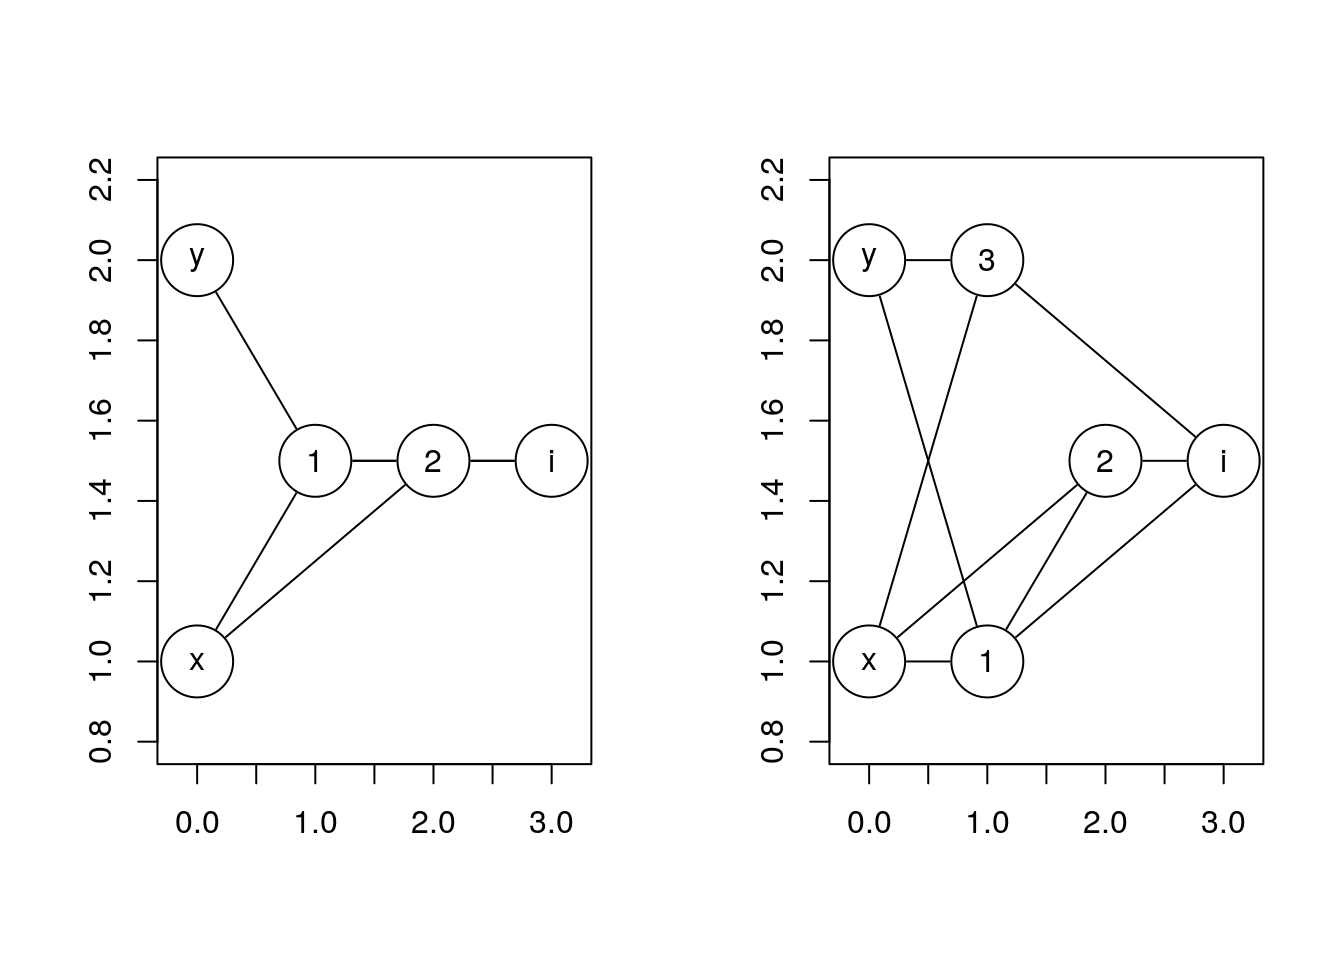
\includegraphics{mayprojtest_files/figure-latex/unnamed-chunk-9-1.pdf}

\end{document}
